\documentclass{article}
\usepackage{fontspec}
\pagestyle{empty}
\usepackage{geometry}
\geometry{paperwidth=40mm, paperheight=40mm, left=2mm, top=0mm, right=2mm, bottom=0mm}
\parindent=0pt
\usepackage{color}
\usepackage{xcolor}
\usepackage{tikz}

\begin{document}
\centering
\vspace*{\fill} \vspace*{-5ex}

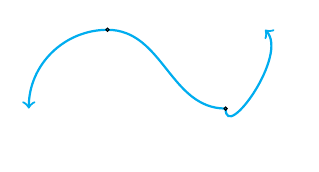
\begin{tikzpicture}
\draw [<->,thick, cyan] (0,0) to [out=90,in=180] (1,1)
to [out=0,in=180] (2.5,0) to [out=-90,in=-45] (3,1) ;
\draw (1, 1) circle(0.02cm);
\draw (2.5, 0) circle(0.02cm);
\end{tikzpicture}

\vspace*{\fill} 
\end{document}%curveinout